
\section{Details of the demographic model}
\label{apx:demographic_model}


Throughout we use in many ways the {\em branching process approximation} --
if an allele is locally rare, then for at least a few generations,
the fates of each offspring are nearly independent.
So, if the allele is locally deleterious, the total numbers of that allele behave as a subcritical branching process,
destined for ultimate extinction.
On the other hand, if the allele is advantageous,
it will either die out or become locally common, with its fate determined in the first few generations.
If the number of offspring of an individual with this allele is the random variable $X$, 
with mean $\E[X] = 1+s$ (selective advantage $s>0$), variance $\var[X]=\xi^2$, and $\P\{X=0\}>0$ (some chance of leaving no offspring),
then the probability of local nonextinction $p_*$ is approximately $p_* \approx 2s/\xi^2$ to second order in $s$.
The precise value can be found by defining the generating function $\Phi(u) = \E[u^X]$; 
the probability of local nonextinction $p_*$ is the minimal solution to $\Phi(1-u) = 1-u$.
(This can be seen because: $1-p_*$ is the probability that an individual's family dies out;
this is equal to the probability that the families of all that individuals' children die out;
since each child's family behaves independently, if the individual has $x$ offspring, this is equal to $(1-p_*)^x$;
and $\Phi(1-p_*) = \E[(1-p_*)^X]$.)


If the selective advantage ($s$) depends on geographic location, 
a similar fact holds: index spatial location by $i \in 1, \ldots, n$,
and for $u = (u_1,u_2,\ldots,u_n)$ define the functions $\Phi_i(u) = \E[ \prod_j u_j^{X_{ij}} ]$,
where $X_{ij}$ is the (random) number of offspring that an individual at $i$ produces at location $j$.
Then $p_* = (p_{*1}, \ldots, p_{*n})$, the vector of probabilities that a new mutation at each location eventually fixes,
is the minimal solution to $\Phi(1-p_*) = 1-p_*$,
i.e.\ $\Phi_i(1-p_*) = 1-p_{*i}$.

%%%%% in rcode/maize_calcs.R
% # maize
% N <- 103359  # plants per field
% Nf <- 561    # ears to make next generation
% e <- 0.068   # prob of total seed stock replacement
% mg <- .0083  # pollen migration
% pm <- .02    # prob of partial stock addition
% m <- 0.2     # proportion of stock replaced
% eqvals <- c(1, iterroot( function (p) { 
%             p.dead <- e + (1/2)*(1-e)*(1-Nf/N)
%             return( p.dead * 1 + 
%                     (1/2)*(1-e)*exp(((1+sb)/p.dead)*( p - 1 )) + 
%                     ((1/2)*(1-e)*Nf/N)*exp(((N/Nf)*(1+sb)/(1-e))*( p - 1 )) 
%                 )
%         } ) )
% genfn <- function (f,selx,migr=.5) { 
%         (e + (1/2)*(1-e)*(1-Nf/N))* 1 + #  no offspring
%         (1/2)*(1-e)*exp(((1+selx)/(1-e))*( f + migr*diff(c(eqvals[1],f,eqvals[2]),differences=2) - 1 )) + # pollen, Poisson mean 1+s(x)
%         (1/2)*(1-e)*(Nf/N)*exp(((N/Nf)*(1+selx/(1-e)))*( f + migr*diff(c(eqvals[1],f,eqvals[2]),differences=2) - 1 )) # seed, Poisson mean (1+s(x))*N/Nf
%     }

Here we consider a linear habitat, so that the selection coefficient at location $\ell_i$ is $s_i = \min( s_b, \max( - s_d, \alpha \ell_i ) )$.
There does not seem to be a nice analytic expression for $p_*$ in this case,
but since $1-p_*$ is a fixed point of $\Phi$, the solution can be found by iteration:
$1-p_* = \lim_{n \to \infty} \Phi^n(u)$ for an appropriate starting point $u$.

\subsection{Maize model}

Specifically, the migration and reproduction dynamics we use are as follows.
On a large scale,
fields of $N$ plants are replanted each year from $N_f$ ears,
either from completely new stock (with probability $p_e$),
from partially new stock (a proportion $r_m$ with probability $p_m$),
or entirely from the same field.
Plants have an average of $\mu_E$ ears per plant, and ears have an average of $N/N_f$ kernels;
so a plant has on average $\mu_E N/N_f$ kernels, and a field has on average $\mu_E N$ ears and $\mu_E N^2/N_f$ kernels.
We suppose that a plant with the selected allele is pollen parent to $(1+s) \mu_E N/N_f$ kernels,
and also seed parent to $(1+s)\mu_E N/N_f$ kernels, still in $\mu_E$ ears.
The number of offspring a plant has depends on how many of its offspring kernels get replanted.
Some proportion $m_g$ of the pollen-parent kernels are in other fields, and may be replanted;
but with probability $p_e$ no other kernels (i.e.~those in the same field) are replanted.
Otherwise, with probability $1-p_m$ the farmer chooses $N_f$ of the ears from this field to replant
(or, $(1-r_m) N_f$ of them, with probability $p_m$);
this results in a mean number $N_f/N$ (or, $(1-r_m)N_f/N$) of the plant's ears of seed children being chosen,
and a mean number $1+s$ of the plant's pollen children kernels being chosen.
Furthermore, the field is used to completely (or partially) replant another's field with chance $p_e/(1-p_e)$ (or $p_m$);
resulting in another $N_f/N$ (or $r_m N_f/N$) ears and $1+s$ (or $r_m (1+s)$) pollen children being replanted elsewhere.
Here we have assumed that pollen is well-mixed within a field,
and that the selected allele is locally rare.
Finally, we must divide all these offspring numbers by 2,
since we look at the offspring carrying a particular haplotype, not of the diploid plant's genome.

The above gives mean values; to get a probability model we assume that every count in sight is Poisson.
In other words, we suppose that the number of pollen children is Poisson with random mean $\lambda_P$,
and the number of seed children is a mixture of $K$ independent Poissons with mean $(1+s)N/N_f$ each,
where $K$ is the random number of ears chosen to replant, which is itself Poisson with mean $\mu_K$.
By Poisson additivity, the numbers of local and migrant offspring are Poisson,
with means $\lambda_P = \lambda_{PL} + \lambda_{PM}$ and $\mu_K = \mu_{KL} + \mu_{KM}$ respectively.
With probability $p_e$, $\lambda_{PM} = m_g(1+s)$ and $\mu_K = \lambda_{PL} = 0$.
Otherwise, with probability $(1-p_e)(1-p_m)$, $\mu_{KL} = N_f/N$ and $\lambda_{PL} = (1+s)(1-m_g)$;
and with probability $(1-p_e)p_m$, $\mu_{KL} = (1-r_m) N_f/N$ and $\lambda_{PL} = (1-r_m)(1+s)(1-m_g)$.
The migrant means are,
with probability $(1-p_e) p_e/(1-p_e) = p_e$, $\mu_{KM} = N_f/N$ and $\lambda_{PM} = 1+s$;
while with probability $(1-p_e) p_m$, $\mu_{KM} = r_m N_f/N$ and $\lambda_{PM} = (1+s)(r_m(1-m_g) + m_g)$,
and otherwise $\mu_{KM} = 0$ and $\lambda_{PM} = m_g(1+s)$.


\begin{table}[htb!!]
  \begin{center}
  \begin{tabular}{|cll|}
    \hline
    complete seed stock replacement prob & $p_e$     & 0.068 \\
    pollen migration rate                & $m_g$      & 0.0083 \\
    number of plants per field           & $N$        & $10^5$ \\
    number of ears used to replant       & $N_f$      & 561 \\
    mean ears per plant                  & $\mu_E$    & 3 \\
    partial stock replacement prob       & $p_m$      & 0.02 \\
    mean proportion stock replaced       & $r_m$      & 0.2 \\
    pollen migration distance            & $\sigma_p$ & 0 km \\
    seed replacement distance            & $\sigma_s$ & 50 km \\
    distance between demes               & $a$        & 15 km \\
    width of altitudinal cline           & $w$        & 62km \\
    deleterious selection coefficient    & $s_d$      & varies \\
    beneficial selection coefficient     & $s_b$      & varies \\
    slope of selection gradient          & $\alpha$   & $(s_d+s_b)/w$ \\
    variance in offspring number         & $\xi^2$    & varies \\
    maize population density             & $\rho$     & $5 \times 10^3$ \\
    area of highland habitat             & $A$        & 500 km$^2$ \\
    mean dispersal distance              & $\sigma$   & 1.8 km \\
    \hline 
  \end{tabular}
\end{center}
  \caption{Parameter estimates used in calculations, and other notation.
  \label{tab:parameters}
  }
\end{table}


\subsection{Math}

The generating function of a Poisson with mean $\lambda$ is $\phi(u;\lambda)=\exp(\lambda(u-1))$,
and the generating function of a Poisson($\mu$) sum of Poisson($\lambda$) values is $\phi(\phi(u;\lambda);\mu)$.
Therefore, the generating function for the diploid process, ignoring spatial structure,
is
\begin{align}
 \Phi(u) &= \begin{aligned}[t]
   & p_e \phi(u;m_g(1+s)) \\
   & \quad {} + \left\{ (1-p_e) (1-p_m) \phi(u;(1+s)(1-m_g))\phi(\phi(u;(1+s)N/N_f);N_f/N) \right. \\
   & \quad \qquad \left. {} + (1-p_e) p_m \phi(u;(1+s)(1-r_m)(1-m_g)) \phi(\phi(u;(1+s)N/N_f);(1-r_m)N_f/N) \right\} \\
   & \quad \quad {} \times \left\{ p_e/(1-p_e) \phi(u;1+s) \phi(\phi(u;(1+s)N_f/N);N_f/N) \right. \\
   & \quad \qquad \left. {} + p_m \phi(u;(1+s)(r_m(1-p_e)(1-m_g)+m_g)) \right. \\ 
   & \quad \qquad \quad \left. {}\times \phi(\phi(u;(1+s)N/N_f);r_m N_f/N)\right. \\
   & \quad \qquad \left. {} + (1 - p_e/(1-p_e)-p_m) \phi(u;m_g(1+s)) \right\}
 \end{aligned} \label{eqn:genfn} \\
 &= \begin{aligned}[t]
   & \phi(u;m_g(1+s)) \big( \; p_e \big.\\
   & \quad {} + \left\{ (1-p_e) (1-p_m) \phi(u;(1+s)(1-m_g))\phi(\phi(u;(1+s)N/N_f);N_f/N) \right. \\
   & \quad \qquad \left. {} + (1-p_e) p_m \phi(u;(1+s)(1-r_m)(1-m_g)) \phi(\phi(u;(1+s)N/N_f);(1-r_m)N_f/N) \right\} \\
   & \quad \quad {} \times \left\{ p_e/(1-p_e) \phi(u;(1+s)(1-m_g)) \phi(\phi(u;(1+s)N_f/N);N_f/N) \right. \\
   & \quad \qquad {} + p_m \phi(u;(1+s)r_m(1-m_g)) \\
   & \quad \qquad \quad {} \times \phi(\phi(u;(1+s)N/N_f);r_m N_f/N) \\
   & \quad \qquad \left. {} + (1-p_e/(1-p_e)-p_m) \right\}  \big)
 \end{aligned}
\end{align}
To get the generating function for a haploid, replace every instance of $1+s$ by $(1+s)/2$.

As a quick check,
% \begin{align}
%   \Phi(0) &= p_e + \left\{ (1-p_e)(1-p_m)+(1-p_e)p_m \right\}
%     \times \left\{ p_e/(1-p_e) + p_m + (1-p_e/(1-p_e)-p_m) \right\}
%   &= p_e + (1-p_e)
%   &= 1 .
% \end{align}
% And, 
the mean total number of offspring of a diploid is
\begin{align}
  & \begin{aligned}
(1+s) \big(
    m_g
    + & (1-p_e)\left\{ (1-p_m) ( (1-m_g) + 1 ) + p_m ( (1-r_m)(1-m_g) + (1-r_m) ) \right\} \\
    & \qquad + \left\{ p_e ( (1-m_g) + 1 ) + p_m (1-p_e)( r_m(1-m_g) + r_m ) \right\} 
    \big) 
  \end{aligned}  \\
& \qquad = 
    (1+s) \big( m_g + 
      (1-p_e)(2-m_g)(1 - p_m r_m)
      + ( p_e (2-m_g) + p_m r_m (1-p_e)(2-m_g) )
    \big) \\
& \qquad = (1+s) \big( 
    m_g + (2-m_g) ( (1-p_e) (1 - p_m r_m) + p_e + p_m r_m(1-p_e) )
  \big) \\
& \qquad = (1+s) \big( 
    m_g + (2-m_g)
  \big) \\
& \qquad = 2(1+s) .
\end{align}
Check!

We show numerically later that the probability of establishment is very close to $2s$ over the variance in reproductive number (as expected).
It is possible to write down an expression for the variance, but it's a big, ugly one that doesn't lend itself to intuition.

\subsection{Migration and spatial structure}

To incorporate spatial structure, suppose that the locations $\ell_k$ are arranged in a regular grid, so that $\ell_k = a k$. 
Recall that $s_k$ is the selection coefficient at location $k$.
If the total number of offspring produced by an individual at $\ell_i$ is Poisson($\lambda_i$), with each offspring independently migrating to location $j$
with probability $m_{ij}$,
then the number of offspring at $j$ is Poisson($m_{ij}\lambda_i$),
and so the generating function is
\begin{align}
  \phi(u;\lambda,m) &= \prod_j \exp( \lambda_i m_{ij} ( u_j - 1 ) ) \\
  &= \exp\left\{ \lambda_i \left(\left(\sum_j m_{ij} u_j\right) - 1\right) \right\} .
\end{align}
We can then substitute this expression into equation \eqref{eqn:genfn},
with appropriate migration kernels for pollen and seed dispersal.

For migration, we need migration rates and migration distances for both wind-blown pollen
and for farmer seed exchange.
The rates are parameterized as above;
we need the typical dispersal distances, however.
One option is to say that the typical distance between villages is $d_v$,
and that villages are discrete demes,
so that pollen stays within the deme (pollen migration distance 0)
and seed is exchanged with others from nearby villages;
on average $\sigma_s$ distance away in a random direction.
The number of villages away the seed comes from could be geometric 
(including the possibility of coming from the same village).

\subsection{Dispersal distance}

The dispersal distance
-- the mean distance between parent and offspring --
is the average of the pollen and seed mean dispersal distances.
With the above assumptions, the pollen dispersal distance is zero,
and the seed dispersal distance is the chance of inter-village movement
multiplied by the mean distance moved.
This is
% pe <- .068; pm <- .02; rm <- .2; sigma.s <- 50
% (1/2) * (pe + (1-pe)*pm*rm) * sigma.s
\begin{align}
  \sigma = \frac{1}{2} (p_e + (1-p_e) p_m r_m ) \sigma_s = 1.7932 \text{km}
\end{align}
at the parameter values above.

\subsection{Results}

Iterating the generating function above finds the probability of establishment as a function of distance along the cline.
This is shown in figure \ref{fig:prob_estab}.
Note that the approximation $2s$ divided by the variance in offspring number is pretty darn close.

\begin{figure}[ht!!]
  \begin{center}
    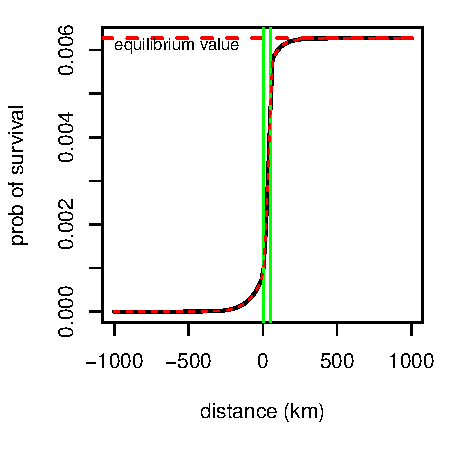
\includegraphics{prob-estab-62}
    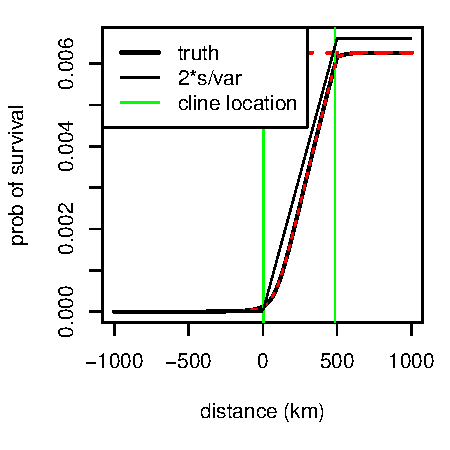
\includegraphics{prob-estab-500}
  \end{center}
  \caption{
  \plr{make this look better}
  Probability of establishment, as a function of distance along and around an altitudinal cline, whise boundaries are marked by the green lines.
  {\bf (A)} The parameters above; with cline width 62km; {\bf (B)} the same, except with cline width 500km.
  \label{sfig:prob_estab}
  }
\end{figure}


%%%%%%%
\section{Adaptation by mutation}

\plr{just a placeholder for now; to be merged in}

First, we'd like to compute how difficult is it for the beneficial adaptation to arise by new mutation.
The rate of appearance of mutant alleles is a Poisson process,
and we can assume that each is successful or not independently,
so the time until the new mutant appears and fixes is exponentially distributed,
with rate equal to the mutation rate multiplied by the probability of establishment integrated over the population.
Referring to figure~\ref{fig:prob_estab},
we see that this is pretty close to ( (area of high altitude) $+$ ($1/2$ area of altitudial gradient) ) $\times$ (population density) $\times$ (prob of establishment at high altitude).

Let $A$ denote (area of high altitude) plus ($1/2$ area of altitudial gradient).
The population density $\rho$ is roughly
0.5--5 people per km$^2$
$\times$ (0.5 ha field/person)
$\times$ (2$\times10^4$ plants per field ha)
$=$ (5000--50000 plants per km$^2$).
As a check, the other set of numbers was
``one village per 15 km''; i.e.\ per square with 15km on a side,
which is 0.444 people per km$^2$.

Since the probability of establishment at high altitude is approximately $2 s_b / \xi^2$, 
with $\xi^2$ the variance in offspring number,
the rate of appearance is just 
\begin{align*}
  \mutrate = 2 \rho A s_b \mu / \xi^2 .
\end{align*}
% rho <- 5000; sb <- 10^(-(1:3)); xisq <- 50; A <- 500
% sapply( c(1e-8,1e-5), function (mu) 2 * rho * A * sb *mu / xisq )
At the values above, with $.1 \le s_b \le .001$, the factor $2 \rho A s_b / \xi^2$ multiplying the mutation rate
varies between $10^2$ and $10^5$,
implying that a single-base mutation with $\mu=10^{-8}$ would have to wait between $10^4$ and $10^6$ generations to fix,
but a mutation with a larger target, say $\mu=10^{-5}$, would fix in tens to thousands of generations, depending on the selection coefficient.



%%%%%%%
\section{Adaptation by migration}

As we show in the theory paper, 
the rate of adaptation by diffusive migration is roughly
\begin{align*}
  \migrate = \rho \frac{s_b \sqrt{2 s_m}}{2\xi^2} \exp\left(- \frac{\sqrt{2 s_m}R}{\sigma} \right) .
\end{align*}
We can talk about this more and give some simulations.
But for now, let's interpret.

First note that for $10^{-1} \le s_m \le 10^{-4}$, the value $1/\sqrt{2s_m}$ is between 2 and 70 --
so the exponential decay of the chance of migration fallws off on a scale of between 2 and 70 times the dispersal distance.
Above we have estimated the dispersal distance to be $\sigma \approx 2$ km,
and far below the mean distance $\sigma_s$ to the field that a farmer replants seed from, when this happens,
which we have as $\sigma_s = 50$ km.
Taking $\sigma=2$ km, we have that $4 \le \sigma/\sqrt{2s_m} \le 150$ km.
A very conservative upper bound might be $\sigma \le \sigma_s/20$ (if farmers replaced 10\% of their seed with long-distance seed every year).
At this upper bound, we would have $5 \le \sigma/\sqrt{2s_m} \le 175$ km,
which is not very different.
This makes the exponential term very small since $R$ is on the order of 1,000 km.

Taking $\sigma=2$ km, we then compute that 
% rho <- 5000; sb <- .01; sm <- 10^(-(1:4)); xisq <- 50; sigma <- 2
% sapply( 1000*(1:4), function (R) rho * sb * sqrt(2*sm) / (2 *  xisq) * exp(- sqrt(2*sm)*R/sigma ) )
if $s_m = 10^{-4}$ (very weak selection in the lowlands), then for $R=1,000$ km, the migration rate is $\migrate \le 10^{-5}$,
i.e.\ it would take on the order of 100,000 generations (years) to get a successful migrant only 1,000 km away,
under this model of undirected, diffusive dispersal.
For larger $s_m$, the migration rate is much smaller.


%%%%%%%%%%%%
\section{Conclusion}

It seems unlikely that any alleles that are adaptive in the highlands and deleterious at all in the lowlands
would have transited central America by undirected (diffusive) sharing of seed.
The conclusions could change if we drastically underestimate the rate of very long distance sharing of seed,
e.g.\ if sharing across hundreds of kilometers was common at some point.

Both calculations are very pessimistic about the chance of shared single-base changes through either migration or independent mutation.
However, independent mutations could be expected in kilobase-size targets,
suggesting there might be signal for genes that share adaptive changes.


